% id: 88-05
% book: 100발100중 3-2 기말 · 01 3-2 기말(원의 성질·통계·부록)
% section: 실전 모의고사 1회
% figure: crop:fig-88-05.png
% answer: ②
% answer_source: 답지(빠른정답)
% variant_level: 0 (원본 전사)
% 이 파일은 build.mjs 가 items.json 에서 만든다. 고칠 때는 items.json 을 고친다.
\smash{\raisebox{1.5mm}{\dmkichul{100발100중 3-2 기말 88쪽 05번}}}
다음 중 네 점~$\pt{A}$, $\pt{B}$, $\pt{C}$, $\pt{D}$가 한 원 위에 있지 \underline{않은} 것은? \mbox{[4점]}
\par\smallskip\begin{center}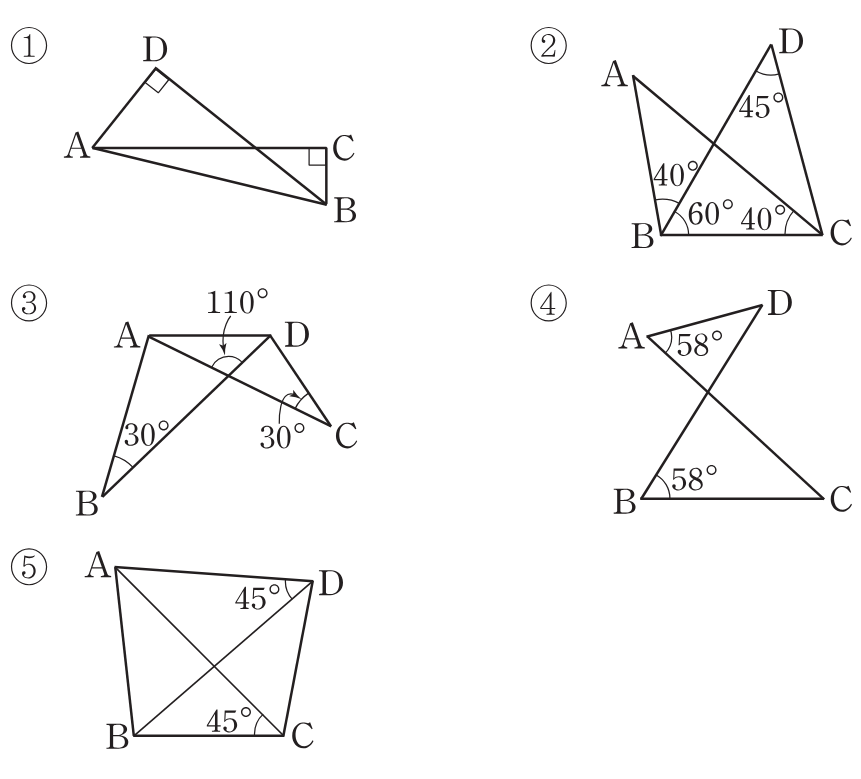
\includegraphics[width=206.6pt]{figures/fig-88-05.png}\end{center}
